\pgfdeclarelayer{background}
\pgfdeclarelayer{foreground}
\pgfdeclarelayer{Beschriftung}
%Farbendefinition
\definecolor{elek}{RGB}{105,105,105}%grau{55,126,184}%blau
\definecolor{pneu}{RGB}{77,175,74}%grün{pneu}{RGB}{105,105,105}%grau
\definecolor{sens}{RGB}{105,105,105}%grau
\definecolor{dat}{RGB}{105,105,105}%grau
\definecolor{strom}{RGB}{105,105,105}%grau %{0,0,0}%schwarz

\tikzset{wagon/.style={draw = gray, ultra thick, opacity = 0.7}}
\tikzset{seite/.style={opacity = 1}}
\tikzset{elek/.style= {draw = elek, ultra thick, opacity = 1}} %elektrische Komponenten
\tikzset{sens/.style={draw = sens, ultra thick, opacity = 1}} %sensorische Komponenten
\tikzset{pneu/.style={draw = pneu, ultra thick, opacity = 1}} %pneumatische Komponenten
\tikzset{dat/.style={draw = dat, ultra thick, opacity = 1}} %Datenkomponenten
\tikzset{strom/.style={draw = strom, ultra thick, opacity = 1}} %Strom- und Datenleitungen
\tikzset{annotation/.style={draw = black, thick, opacity = 0.7, font=\scriptsize}}

\pgfsetlayers{background,main,Beschriftung,foreground}
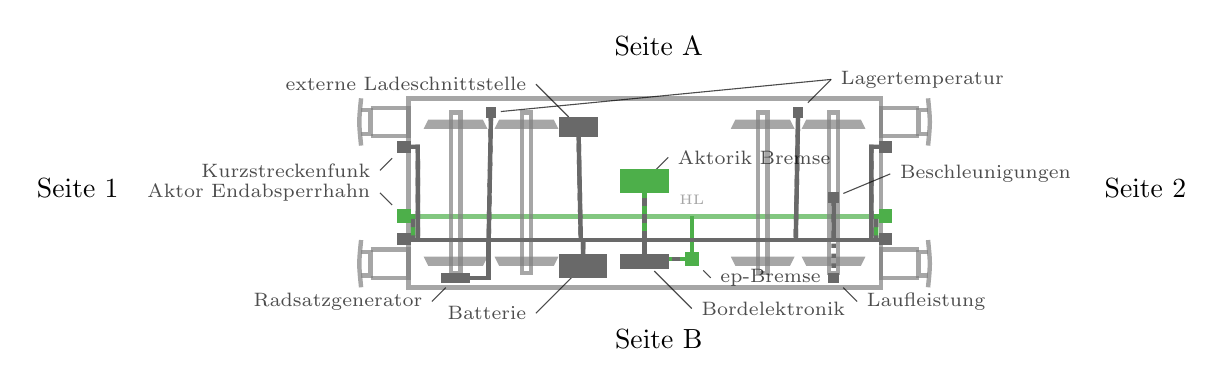
\begin{tikzpicture}[scale=0.6]
%%%%%%%%%%%%%%%%%%%%%%%%%%%%%%%%%%%%%%%%%%%%%%%% Hintergrund %%%%%%%%%%%%%%%%%%%%%%%%%%%%%%%%%%%%%%%%%%%%%
    \begin{pgfonlayer}{background}
    %Seiten
        %Seite A
        \path[seite] (0, 3) rectangle +(.6,.2) node[pos = 0.5] (seiteA) {Seite A};
        %Seite B
        \path[seite] (0, -3.2) rectangle +(.6,.2) node[pos = 0.5] (seiteB) {Seite B};
        %Seite 1
        \path[seite] (-12.3, 0) rectangle +(.6,.2) node[pos = 0.5] (seiteB) {Seite 1};
        %Seite 2
        \path[seite] (10.3, 0) rectangle +(.6,.2) node[pos = 0.5] (seiteB) {Seite 2};      
    %wagon als Basis
    \path[wagon] (-5,-2) -- (-5,2) -- (5,2) -- (5,-2) -- cycle;
    % HL
    \path[wagon, color=pneu] (-5,-.5) -- (5,-.5) node[pos = 0.6, above] {\color{gray} \tiny{HL}};
    % Buffer
    \begin{scope}[shift = {(-5,1.5)}]
    	\path[wagon] (-.8,.3) -- (0,.3) -- (0,-.3) -- (-.8,-.3);
    	\path[wagon] (-1,.25) -- (-.8,.25) -- (-.8,-.25) -- (-1,-.25);
    	\path[wagon] (-1,-.5) .. controls (-1.05,0) and (-1.05,0) .. (-1,.5);
    \end{scope}
    \begin{scope}[shift = {(-5,-1.5)}]
    	\path[wagon] (-.8,.3) -- (0,.3) -- (0,-.3) -- (-.8,-.3);
    	\path[wagon] (-1,.25) -- (-.8,.25) -- (-.8,-.25) -- (-1,-.25);
    	\path[wagon] (-1,-.5) .. controls (-1.05,0) and (-1.05,0) .. (-1,.5);
    \end{scope}
    \begin{scope}[shift = {(5,-1.5)}, rotate = 180]
    	\path[wagon] (-.8,.3) -- (0,.3) -- (0,-.3) -- (-.8,-.3);
    	\path[wagon] (-1,.25) -- (-.8,.25) -- (-.8,-.25) -- (-1,-.25);
    	\path[wagon] (-1,-.5) .. controls (-1.05,0) and (-1.05,0) .. (-1,.5);
    \end{scope}
    \begin{scope}[shift = {(5,1.5)}, rotate = 180]
    	\path[wagon] (-.8,.3) -- (0,.3) -- (0,-.3) -- (-.8,-.3);
    	\path[wagon] (-1,.25) -- (-.8,.25) -- (-.8,-.25) -- (-1,-.25);
    	\path[wagon] (-1,-.5) .. controls (-1.05,0) and (-1.05,0) .. (-1,.5);
    \end{scope}
    %Wheelset
    \begin{scope}[shift = {(-4,0)}]
    	\path[wagon] (-.1,1.7) -- (.1,1.7) -- (.1,-1.7) -- (-.1, -1.7) -- cycle; 
    	\path[wagon] (-.6,1.4) -- (.6,1.4) -- (.55,1.5) -- (-.55, 1.5) -- cycle; 
    	\path[wagon] (-.6,-1.4) -- (.6,-1.4) -- (.55,-1.5) -- (-.55, -1.5) -- cycle; 
    \end{scope}
        \begin{scope}[shift = {(-2.5,0)}]
    	\path[wagon] (-.1,1.7) -- (.1,1.7) -- (.1,-1.7) -- (-.1, -1.7) -- cycle; 
    	\path[wagon] (-.6,1.4) -- (.6,1.4) -- (.55,1.5) -- (-.55, 1.5) -- cycle; 
    	\path[wagon] (-.6,-1.4) -- (.6,-1.4) -- (.55,-1.5) -- (-.55, -1.5) -- cycle; 
    \end{scope}
    \begin{scope}[shift = {(4,0)}]
    	\path[wagon] (-.1,1.7) -- (.1,1.7) -- (.1,-1.7) -- (-.1, -1.7) -- cycle; 
    	\path[wagon] (-.6,1.4) -- (.6,1.4) -- (.55,1.5) -- (-.55, 1.5) -- cycle; 
    	\path[wagon] (-.6,-1.4) -- (.6,-1.4) -- (.55,-1.5) -- (-.55, -1.5) -- cycle; 
    \end{scope}
    \begin{scope}[shift = {(2.5,0)}]
    	\path[wagon] (-.1,1.7) -- (.1,1.7) -- (.1,-1.7) -- (-.1, -1.7) -- cycle; 
    	\path[wagon] (-.6,1.4) -- (.6,1.4) -- (.55,1.5) -- (-.55, 1.5) -- cycle; 
    	\path[wagon] (-.6,-1.4) -- (.6,-1.4) -- (.55,-1.5) -- (-.55, -1.5) -- cycle; 
    \end{scope}
    \end{pgfonlayer}
%%%%%%%%%%%%%%%%%%%%%%%%%%%%%%%%%%%%%%%%%%%%%%% Vordergrung %%%%%%%%%%%%%%%%%%%%%%%%%%%%%%%%%%%%%%%%%%%%%%%%%
    \begin{pgfonlayer}{foreground} %Komponete
    %elektronische Komponenten
        %Radsatzgenerator
        \path[elek, fill = elek, thin] (-4.3, -1.9) rectangle +(.6,.2) node[pos = 0.5] (wsg) {};
        %Rechner
        \path[elek, fill = elek, thin] (-.5, -1.6) rectangle +(1,.3) node[pos = 0.5] (bcu) {};
        %Batterie
        \path[elek, fill = elek, thin] (-1.8, -1.8) rectangle +(1,.5) node[pos = 0.5] (bat) {};
        %optionale Ladeelektronik
        \path[elek, fill = elek, thin] (-1.8, 1.2) rectangle +(0.8,.4) node[pos = 0.5] (ole) {};
    % pneumatische Komponenten
        %epBremse
        \path[pneu, fill = pneu] (.9,-1.3) rectangle (1.1,-1.5) node[pos = 0.5] (epb) {};
        %Endabsperrhähne
        \path[pneu, fill = pneu] (-5.2, -.4) rectangle (-5,-.6) node[pos = 0.5] (eca) {};
        \path[pneu, fill = pneu] (5.2, -.4) rectangle (5,-.6) node[pos = 0.5] (ecb) {};
        %Aktorik Bremse
        \path[pneu, fill = pneu, thin] (-.5, 0) rectangle +(1,.5) node[pos = 0.5] (bcu2) {};
    %sensorische Komponenten
        %drahtloserSensor
        \path[sens, fill = sens, thin] (3.9, -1.7) rectangle +(.2,-.2) node[pos = 0.5] (wss) {};
        %Flachstellendektektor
        \path[sens, fill=sens, thin] (3.15, 1.8) rectangle +(.2,-.2) node[pos = 0.5] (flachstelle) {};
        \path[sens, fill=sens, thin] (-3.35, 1.8) rectangle +(.2,-.2) node[pos = 0.5] (flachstelle2) {};
        %Laufleistung
        \path[sens, fill = sens, thin] (3.9, 0) rectangle +(.2,-.2) node[pos = 0.5] (ll) {};
    %Datenkomponeten
        %Kurzstreckenfunk
        \path[dat, fill = dat] (-5.2, -.9) rectangle (-5,-1.05)node[pos = 0.5] (sra) {};
        \path[dat, fill = dat] (5.2, -.9) rectangle (5,-1.05)node[pos = 0.5] (srb) {};
        \path[dat, fill = dat] (5.2, .9) rectangle (5,1.05)node[pos = 0.5] (src) {};
        \path[dat, fill = dat] (-5.2, .9) rectangle (-5,1.05) node[pos = 0.5] (srd) {};
    \end{pgfonlayer}
%%%%%%%%%%%%%%%%%%%%%%%%%%%%%%%%%%%%%%%%%%%%%%% Beschriftung %%%%%%%%%%%%%%%%%%%%%%%%%%%%%%%%%%%%%%%%%%%%%%%%%
    \begin{pgfonlayer}{Beschriftung}
    %elektronische Komponenten
        %Radsatzgenerator
        \path[annotation, thin] (wsg) -- +(-.5,-.5) node[left] {Radsatzgenerator};
        %Rechner
        \path[annotation, thin] (bcu) -- +(1,-1) node[right] {Bordelektronik};
        %Batterie
        \path[annotation, thin] (bat) -- +(-1,-1) node[left] {Batterie};
        %optionale Ladeelektronik
        \path[annotation, thin] (ole) -- +(-.9,.9) node[left] {externe Ladeschnittstelle};
    %pneumatische Komponenten
        %epBremse
        \path[annotation, thin] (epb) -- +(.4,-.4) node[right] {ep-Bremse};
        %Endabsperrhähne
        \path[annotation, thin] (eca) -- +(-.5,.5) node[left] {Aktor Endabsperrhahn};
        %Aktorik Bremse
        \path[annotation, thin] (bcu2) -- +(.5,.5) node[right] {Aktorik Bremse};
    %sensorische Komponenten
        %drahtloserSensor
        \path[annotation, thin] (wss) -- +(.5,-.5) node[right] {Laufleistung}; 
        %Flachstellen
        \path[annotation, thin] (flachstelle) -- +(.7,.7) node[right] {Lagertemperatur};
        \path[annotation, thin] (flachstelle2) -- +(7.2,.7) node[right] {};
        %Laufleistung
        \path[annotation, thin] (ll) -- +(1.2,.5) node[right] {Beschleunigungen};
    %Datenkomponeten
        %Kurzstreckenfunk
        \path[annotation, thin] (srd) -- +(-.5,-.5) node[left] {Kurzstreckenfunk};    
    \end{pgfonlayer}
%%%%%%%%%%%%%%%%%%%%%%%%%%%%%%%%%%%%%%%%%%%%%% Main %%%%%%%%%%%%%%%%%%%%%%%%%%%%%%%%%%%%%%%%%%%%%%%%%%%%
    \begin{pgfonlayer}{main} %Leitungen
    %elek
        %Radsatzgenerator
        \path[elek] (wsg) +(-.1,0) -| (-3.3, -1);%-- +(1,0) -- (-3.2,-1);
        \path[strom, dashed] (wsg) +(-.1,0) -| (-3.3, -1);%-- +(1,0) -- (-3.2,-1);
        %Rechner
        \path[elek] (bcu) +(0,0)  -- (0,-1);
        \path[strom, dashed] (bcu) +(0,0)  -- (0,-1);
        %Batterie
        \path[elek] (bat) +(0,0)  -- (-1.3,-1);
        \path[strom, dashed] (bat) +(0,0)  -- (-1.3,-1);
        %optionale Ladeelektronik
        \path[elek] (ole) +(0,0)  -- (-1.35,-1);
        \path[strom, dashed] (ole) +(0,0)  -- (-1.35,-1);
    %pneu
        %ep-Bremse
        \path[pneu] (1,-.5) -- (1,-1.3);
        %\path[strom, dashed] (1,-.5) -- (1,-1.3);
        \path[pneu] (epb) +(.1,0) -- +(-.5,0);
        \path[strom, dashed] (epb) +(.1,0) -- +(-.5,0);
        %Endabsperrhähne
        \path[pneu] (eca) +(-.1,0) -- +(.2,0) -- (-4.9,-1);
        \path[strom, dashed] (eca) +(-.1,0) -- +(.2,0) -- (-4.9,-1);
        \path[pneu] (ecb) +(.1,0) -- +(-.2,0) -- (4.9,-1);
        \path[strom, dashed] (ecb) +(.1,0) -- +(-.2,0) -- (4.9,-1);
        %Aktorik Bremse
        \path[pneu] (bcu2) +(0,0)  -- (0,-1);
        \path[strom, dashed] (bcu2) +(0,0)  -- (0,-1);
    %Sensorische Kompoenten
        %Flachstellen
        \path[sens] (flachstelle)+(0,0) -- (3.2, -1);
        \path[strom, dashed] (flachstelle)+(0,0) -- (3.2, -1);
        \path[sens] (flachstelle2) +(0,0)-- (-3.3, -1);
        \path[strom, dashed] (flachstelle2) +(0,0)-- (-3.3, -1);
        %Laufleistung
        \path[sens] (ll)+(0,0) -- (4, -1);
        \path[strom, dashed] (ll)+(0,0) -- (4, -1);
        %drahloser Sensor
        \path[strom, dotted] (wss)+(0,0) -- (4, -1);
    %Strom- und Datenleitung
        \path[dat] (-5,-1) -- (5,-1);
        \path[strom, dashed] (-5,-1) -- (5,-1);
        %Kurzstreckenfunk
        \path[dat] (srd) +(-.1,0) -- +(.3,0) -- (-4.8,-1);
        \path[strom, dashed] (srd) +(-.1,0) -- +(.3,0) -- (-4.8,-1);
        \path[dat] (src) +(.1,0) -- +(-.3,0) -- (4.8,-1);
        \path[strom, dashed] (src) +(.1,0) -- +(-.3,0) -- (4.8,-1);
    \end{pgfonlayer}

\end{tikzpicture}
